\documentclass[english, a4paper,11pt]{article}
\usepackage[utf8]{inputenc}
\usepackage[T1]{fontenc,url} %url
\urlstyle{sf} %sf
\usepackage{babel,textcomp,csquotes, varioref,graphicx, gensymb}
% \usepackage[]{circuitikz}
\usepackage{tikz}
\usetikzlibrary{shapes,arrows}
\usepackage[backend=biber,style=numeric-comp, sortcites]{biblatex}

\bibliography{ref.bib} 

%opening
\title{Complete system test-bench}
\author{Espen Klein Nilsen and \\Vegard Midtbøen}

\begin{document}

\maketitle

\section{System overview}
The overall structure of the system is seen in Figure \ref{block_diagram}.



\tikzstyle{block} = [draw, fill=blue!20, rectangle, 
    minimum height=4em, minimum width=3em]
\tikzstyle{input} = [coordinate]
\tikzstyle{output} = [coordinate]
\tikzstyle{pinstyle} = [pin edge={to-,thin,black}]
\begin{figure}[!ht]
  \begin{tikzpicture}[auto, node distance=2cm,>=latex']
      % We start by placing the blocks
      \node [input, name=input] {};
      \node [block, right of=input, node distance=2cm] (sample_and_hold) {S\&H};
      \node [block, right of=sample_and_hold, node distance=4cm] (comparator) {Comparator};
      \node [block, right of=comparator, node distance=4cm] (sar_logic) {SAR Logic};
      
      % We draw an edge between the controller and system block to 
      % calculate the coordinate xsh(t). We need it to place the measurement block. 
      \draw [->] (sample_and_hold) -- node[name=xsh(t)] {$x_{sh}(t)$} (comparator);
      \draw [->] (comparator) -- node[name=xc(nT)] {$x_{c}(nT)$} (sar_logic);
      \node [block, below of=sar_logic, node distance=3cm] (dac){DAC};
      \node [output, right of=sar_logic, node distance=3cm] (output) {};
    
      % Once the nodes are placed, connecting them is easy. 
      \draw [draw,->] (input) -- node [name=xc(t)] {$x_{c}(t)$}(sample_and_hold);
      \draw [->] (sar_logic) -- node [name=digital_out] {Digital out}(output);
      \draw [->] (sar_logic) -- node [name=nbit] {N-bit} (dac);
      \draw [->] (dac) -| node [name=negfeedback, bend left] {Negative feedback}(comparator);     
  \end{tikzpicture}
  \caption{Block diagram}
  \label{block_diagram}
\end{figure}




\section{Schematic}
We have not completed our research in circuits to use in this project. 
We have created schematics for some simple circuits but we expect that some (or all) of the circuits is going to change.
See test-benches in the next section.

\section*{Schematic: SAR\_system}
The SAR\_system is the complete schematic for the whole system. It consists of a sample and hold block, a comparator block, the SAR logic and the digital-to-analog converter block. Figure 
\ref{sar:system} shows the schematic that has been created.\\
\begin{figure}[!ht]
 \centering
   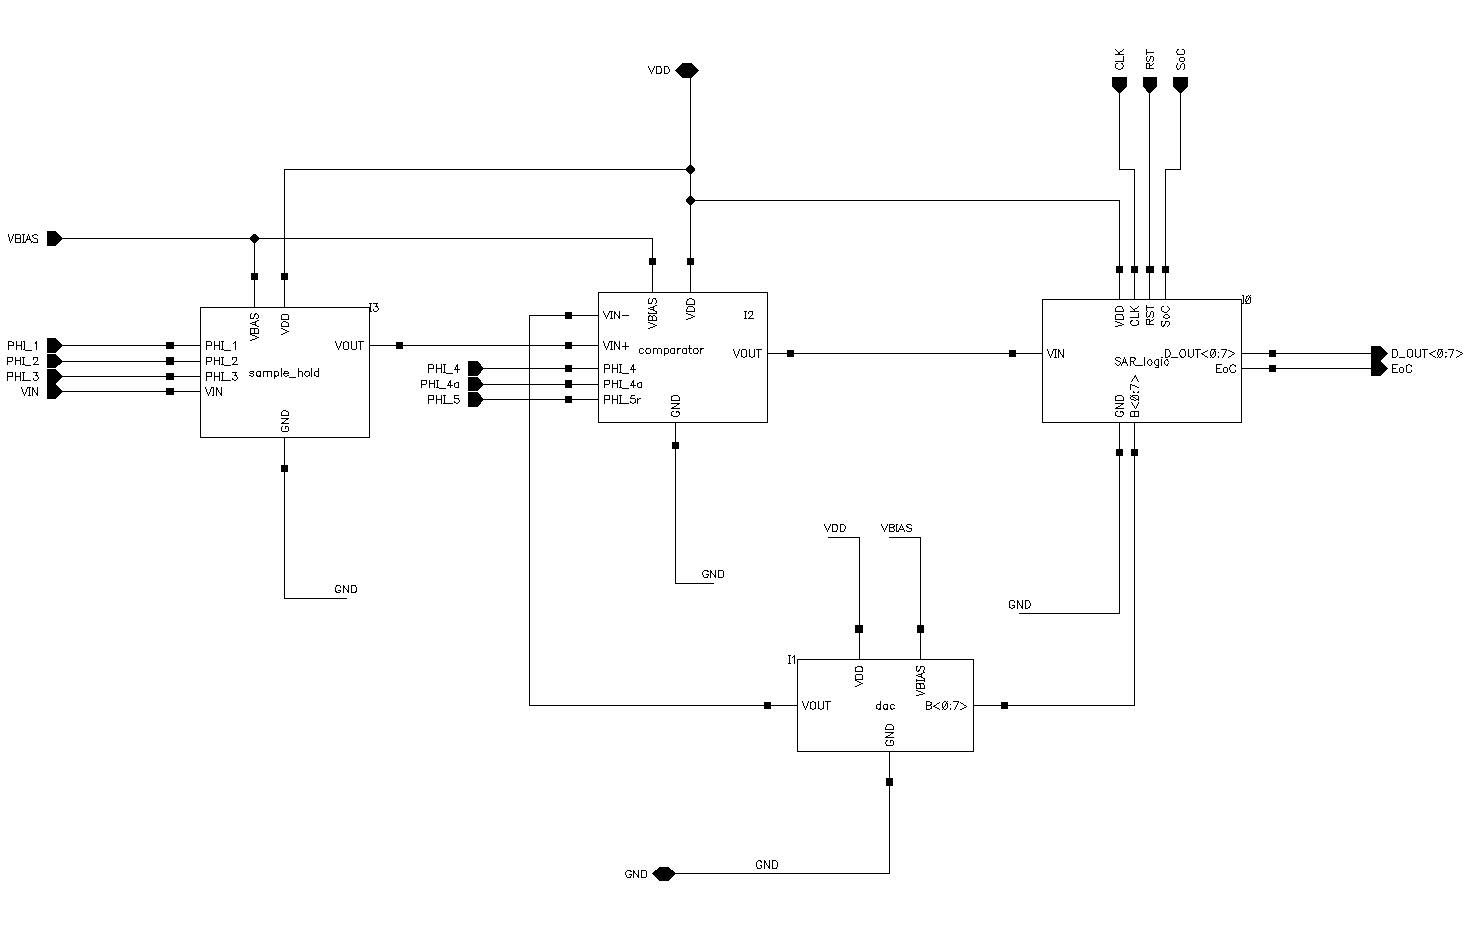
\includegraphics[width=\textwidth]{img/SAR_system}
   \caption{SAR\_system}
   \label{sar:system}
\end{figure}

\section*{Schematic: sample\_hold}
The sample and hold (S/H) is based on a circuit provided by R. Jacob Baker in the book CMOS Mixed-Signal Circuit Design \cite{baker}, and can be seen in Figure \ref{sample:hold}. 
The implementation is a single-ended S/H implementation. When $\phi_{1}$ and $\phi_{2}$ is high, $\phi_{3}$ is low, and the bottom plate of the hold capacitor is charged by the input signal, 
while the top plate is held to ground by the feedback around the opamp. When the $\phi_{2}$ is turned off, its charge will be injected into the low impedance input, VIN, since the impedance 
looking into the left of the $\phi_{2}$ switch is large.\\
\\
This implementation has not yet been tested, and may therefor be changed during the project.\\
\begin{figure}[!ht]
 \centering
   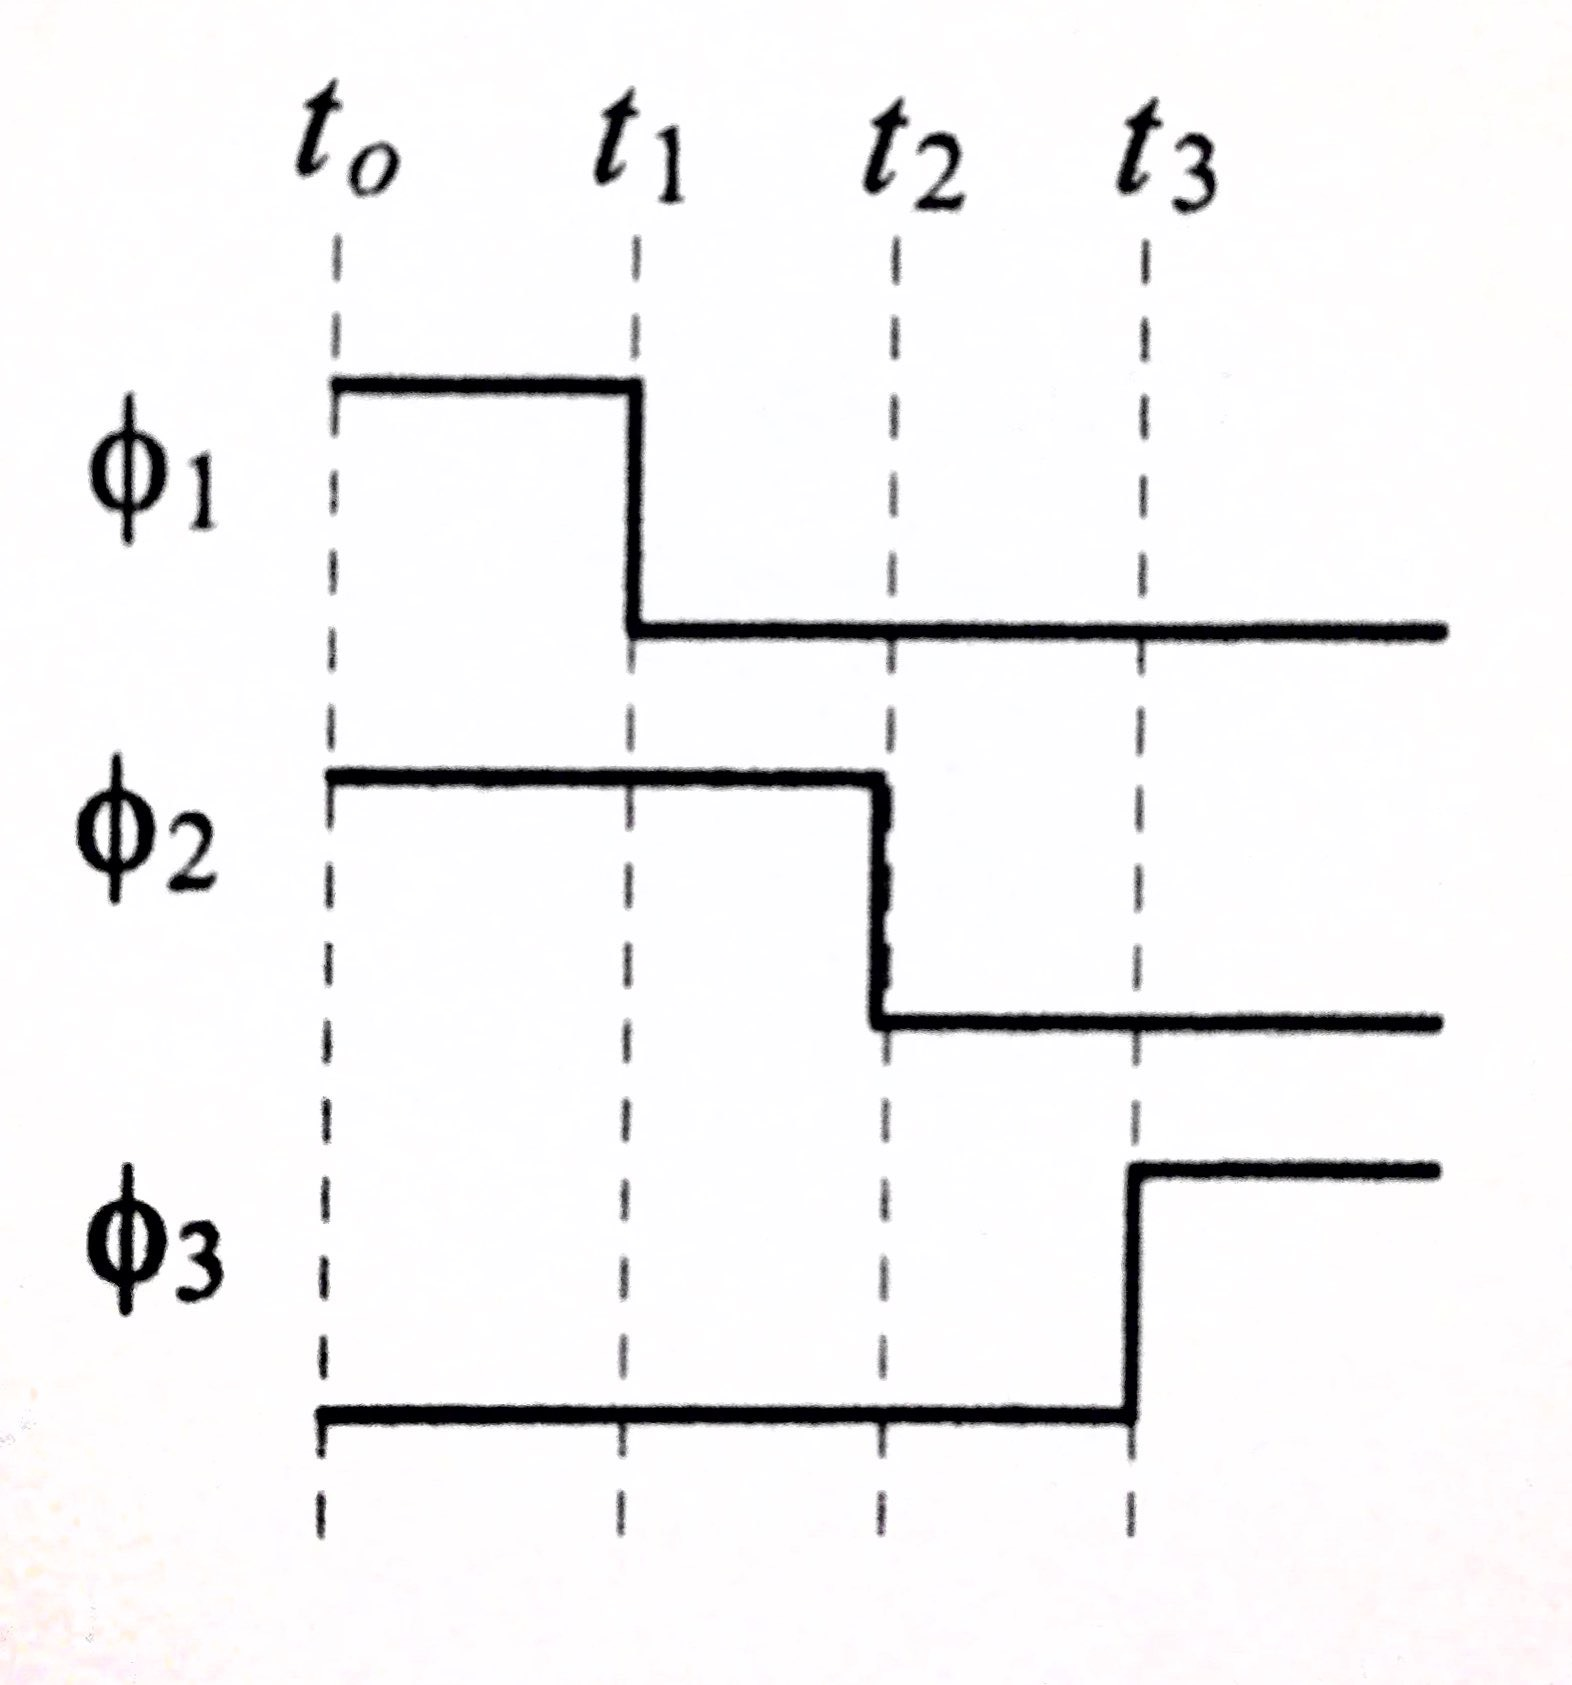
\includegraphics[width=0.3\textwidth]{img/timing_sample_hold.jpg}
   \caption{Single-ended S/H operation \cite{baker}}
   \label{timing}
\end{figure}
\begin{figure}[!ht]
 \centering
   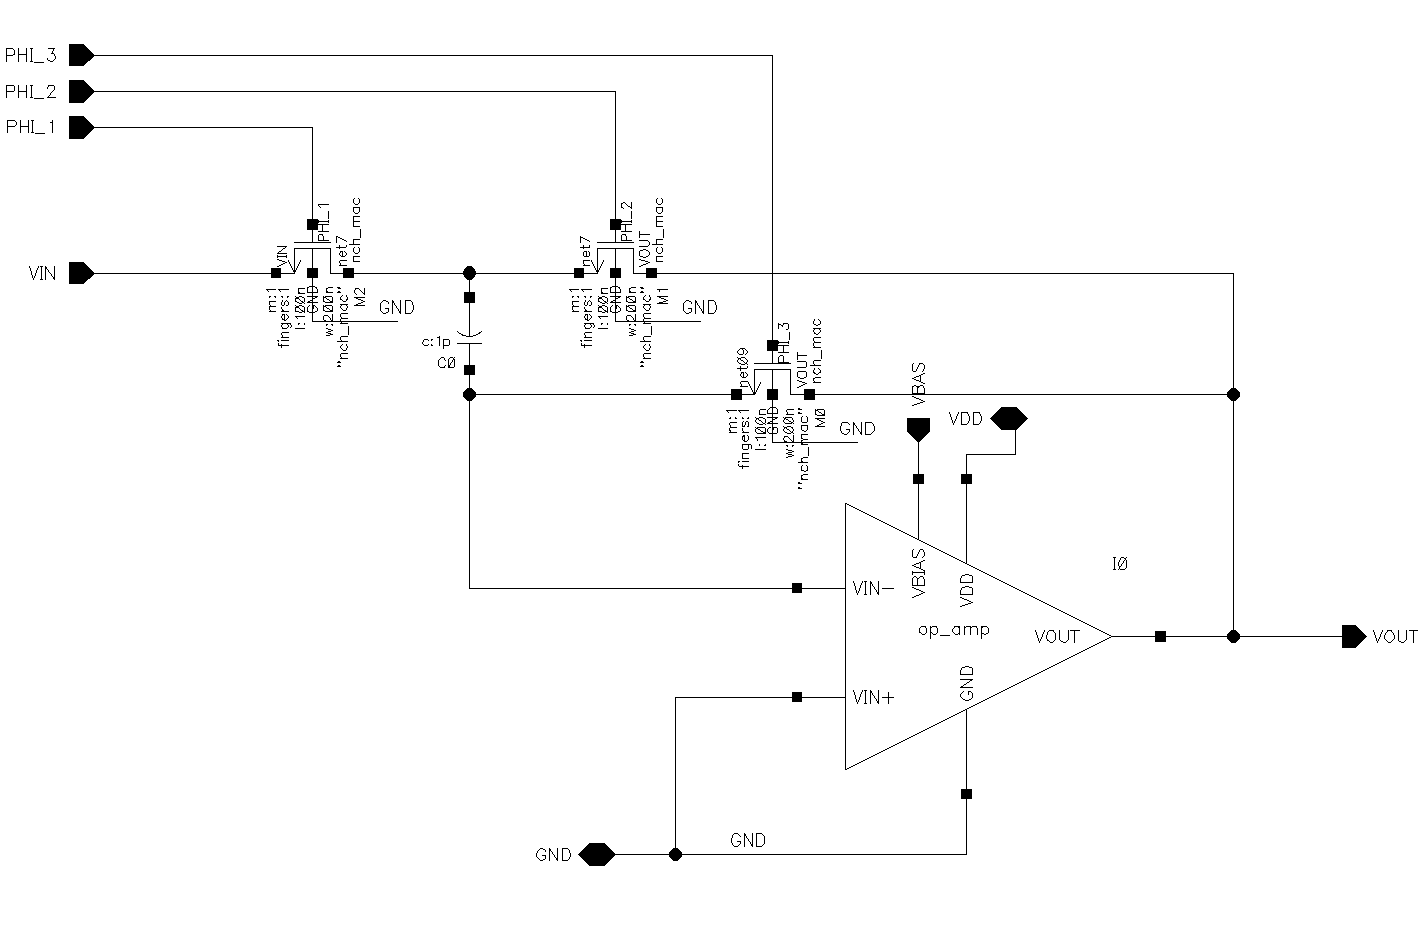
\includegraphics[width=\textwidth]{img/sample_hold}
   \caption{Sample and hold}
   \label{sample:hold}
\end{figure}


\section*{Schematic: comparator}
The design of the comparator is based on a design in the book Analog Integrated Circuit Design by Carusone, Johns and Martin \cite{carusone}, and can be seen in Figure \ref{comparator}. 
\begin{figure}[!ht]
 \centering
   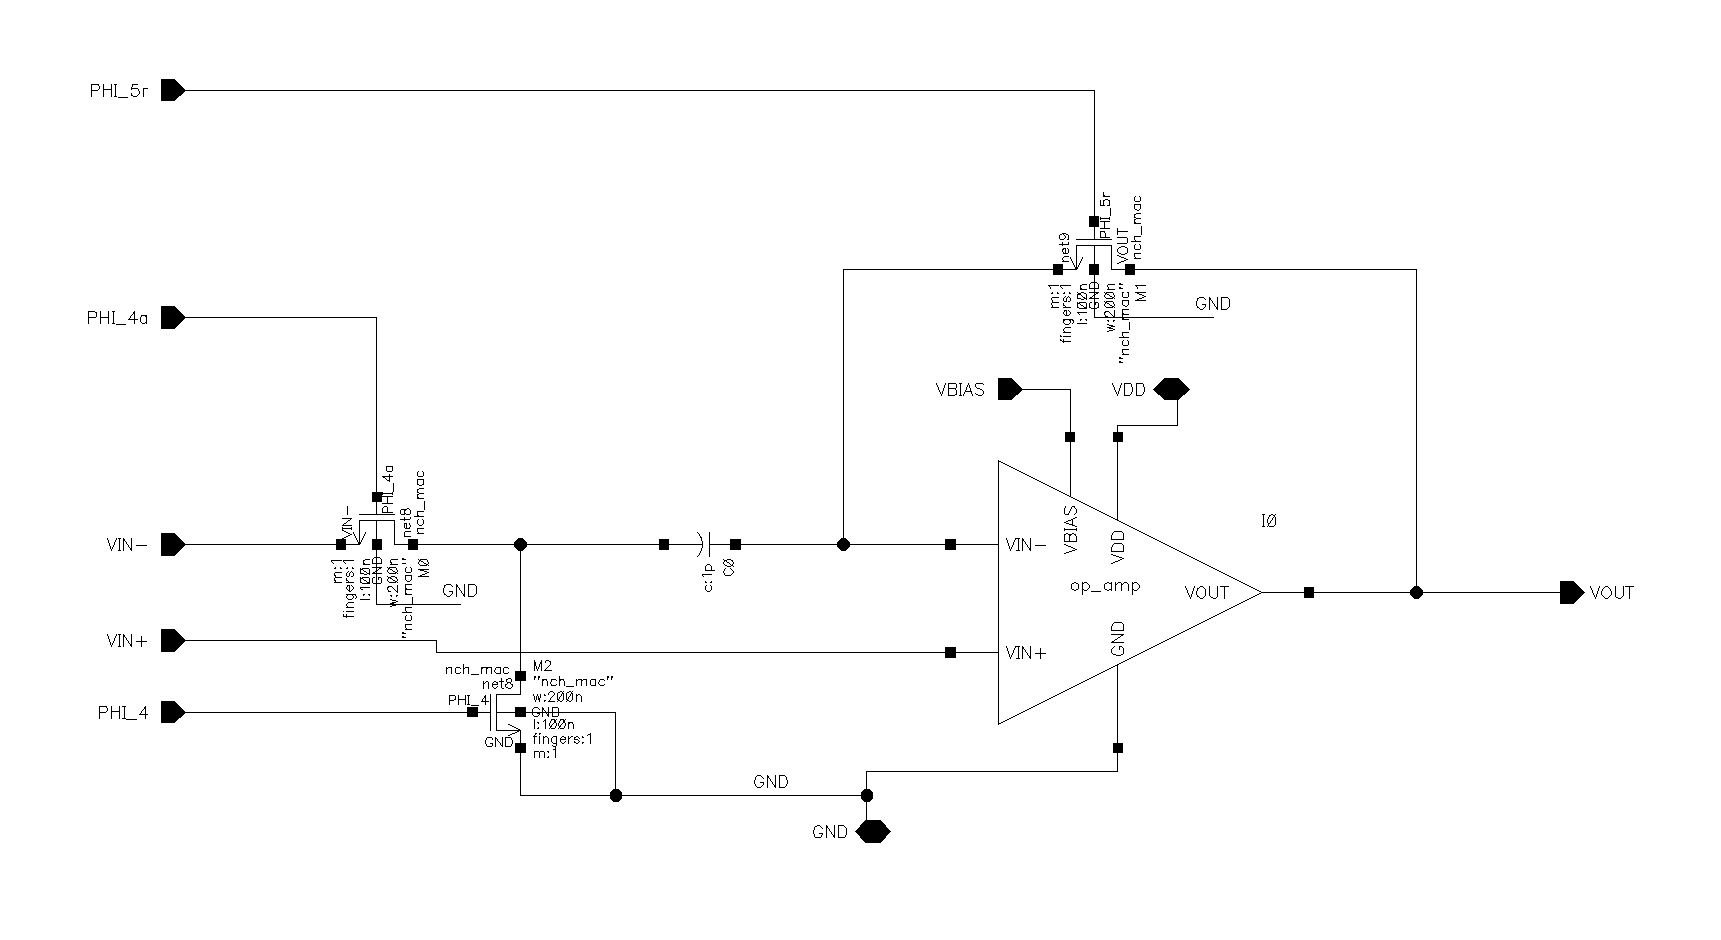
\includegraphics[width=\textwidth]{img/comparator}
   \caption{Comparator}
   \label{comparator}
\end{figure}


\section*{Schematic: SAR\_logic}
% \begin{figure}[!ht]
%  \centering
%    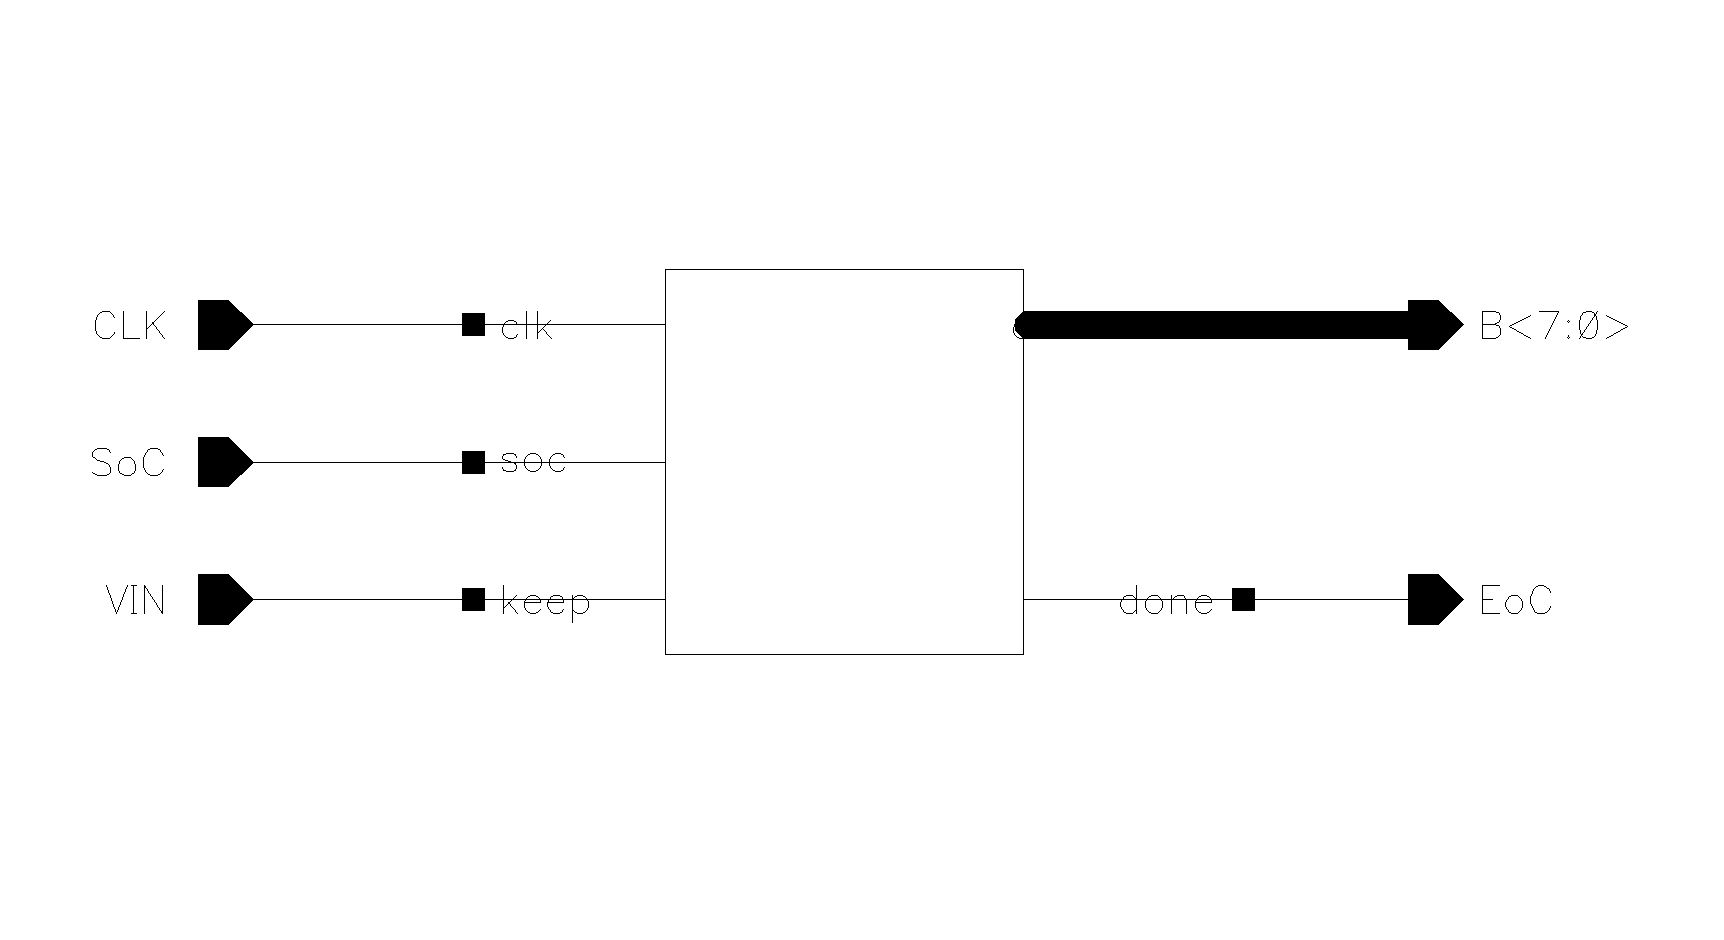
\includegraphics[width=0.4\textwidth]{img/SAR_logic}
%    \caption{Single-ended S/H opartion \cite{CMOS-baker}}
%    \label{timing}
% \end{figure}
We have not completed the schematics for the SAR logic. The chematic for the SAR is therefor not invluded in this document.

\section*{Schematic: dac}
\begin{figure}[!ht]
 \centering
   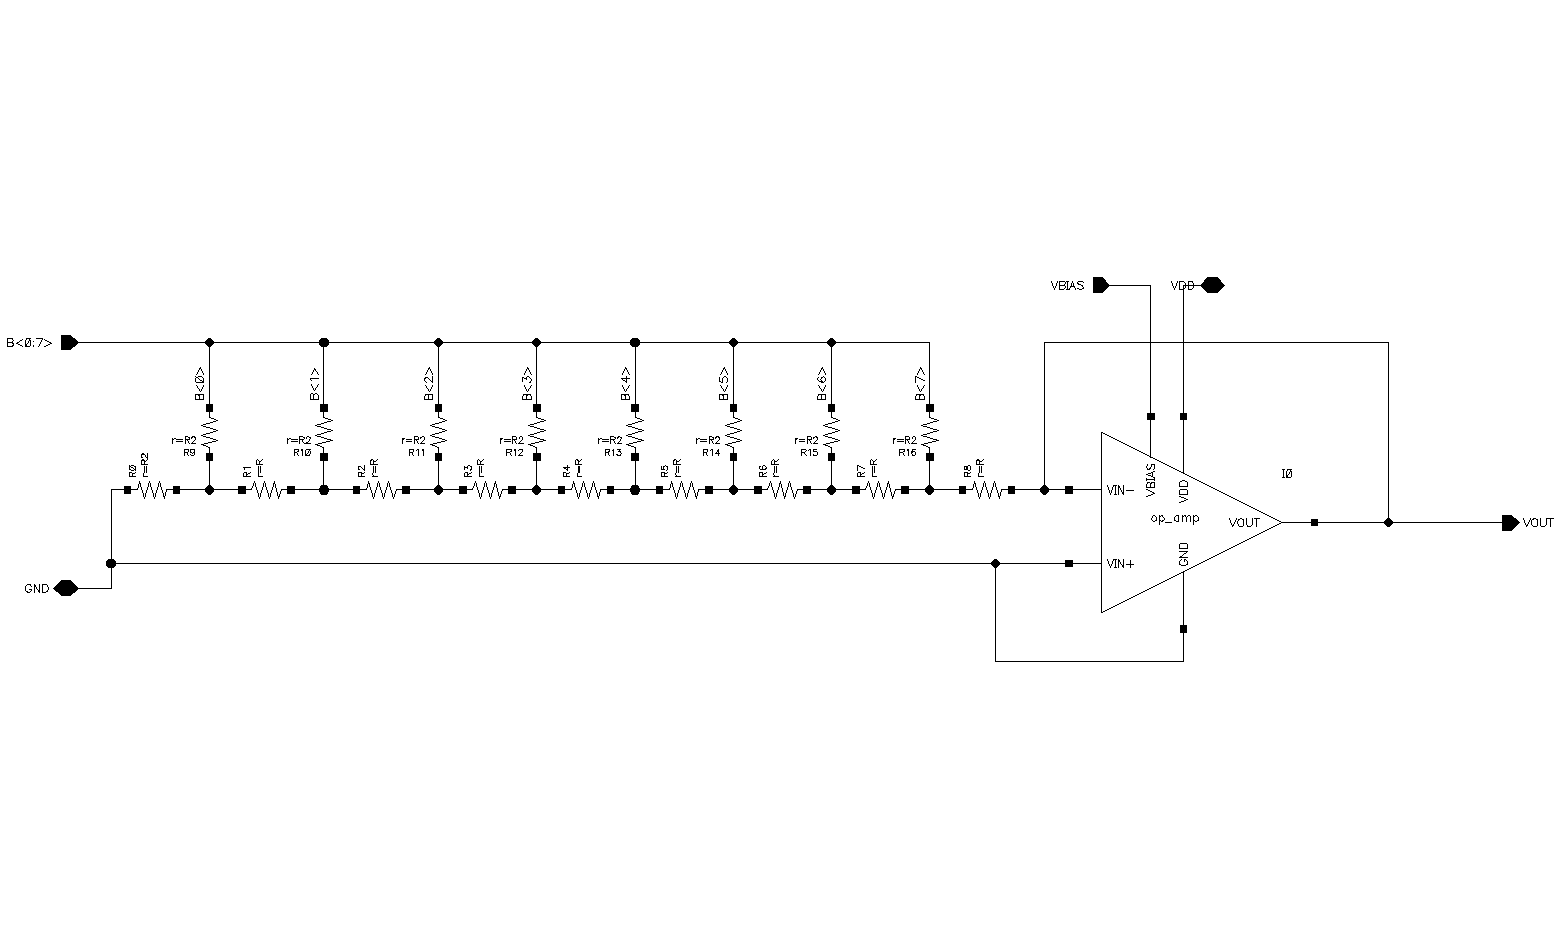
\includegraphics[width=\textwidth]{img/dac}
   \caption{DAC}
   \label{dac}
\end{figure}
This DAC circuit is based on the R-2R ladder from the book Analog Integrated Circuit Design by Carusone, Johns and Martin \cite{carusone}. This design commonly used in many applications, and
is therefor the main reason for why we have chosen to make this design. The DAC schematic can be seen in Figure \ref{dac}.

\section*{Schematic: op\_amp}
The op-amp circuit is based on a design from CMOSedu.com (R. Jacob Baker), and is a commonly used differential pair op-amp. We have tried some different designs, but we have not succeeded in 
any of the other designs. This is not the final version, since it is not fully tested. The dimensions for the NMOS and PMOS transistors are based on a former thesis that R. Jacob Baker has 
referred to in his web-page. For the NMOS and the PMOS, we have used the relation 10/2 and 22/2 respectively \cite{Saxena}. The final design can be seen in Figure \ref{opamp}\\
\\
To test the op-amp, we have made a simple test-bench that can be seen in section \textbf{Schematic: SIM\_op\_amp}.
\begin{figure}[!ht]
 \centering
   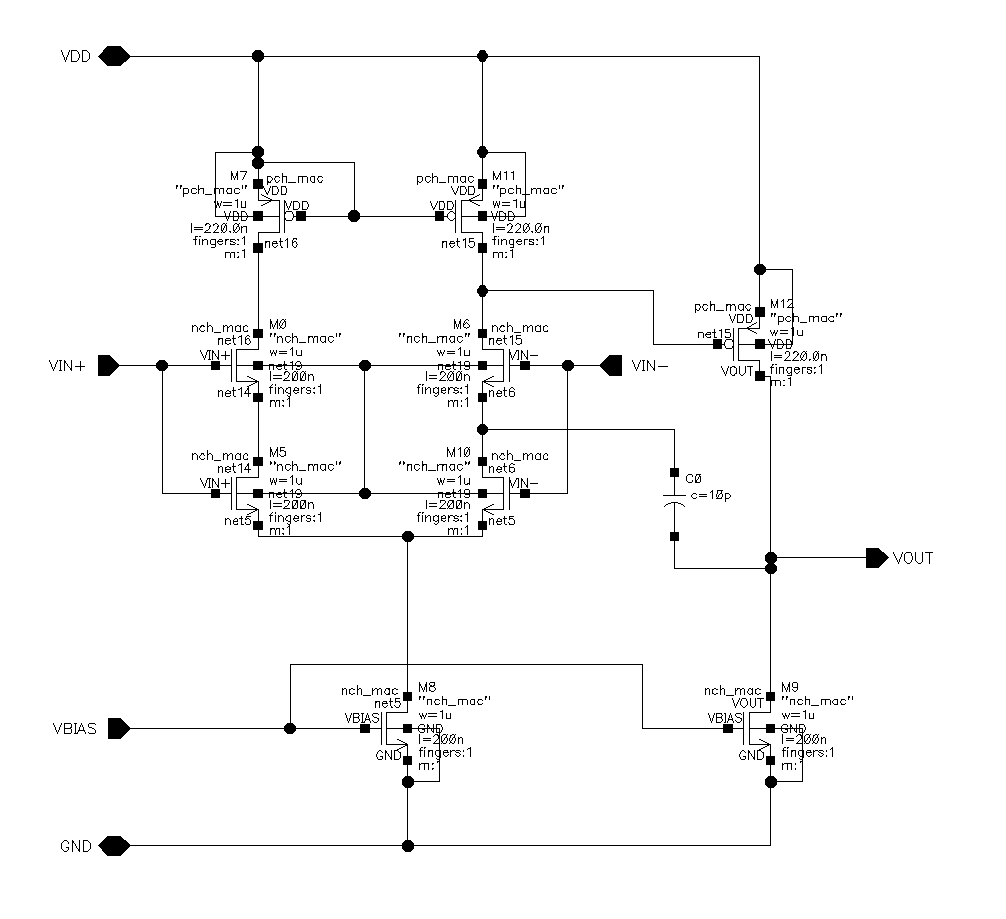
\includegraphics[width=\textwidth]{img/op_amp_3}
   \caption{Opamp}
   \label{op-amp}
\end{figure}


\section{Test bench}
In this section a short overview of the different test-benches for our components is presented.

\section*{Schematic: SIM\_system}
\begin{figure}[!ht]
 \centering
   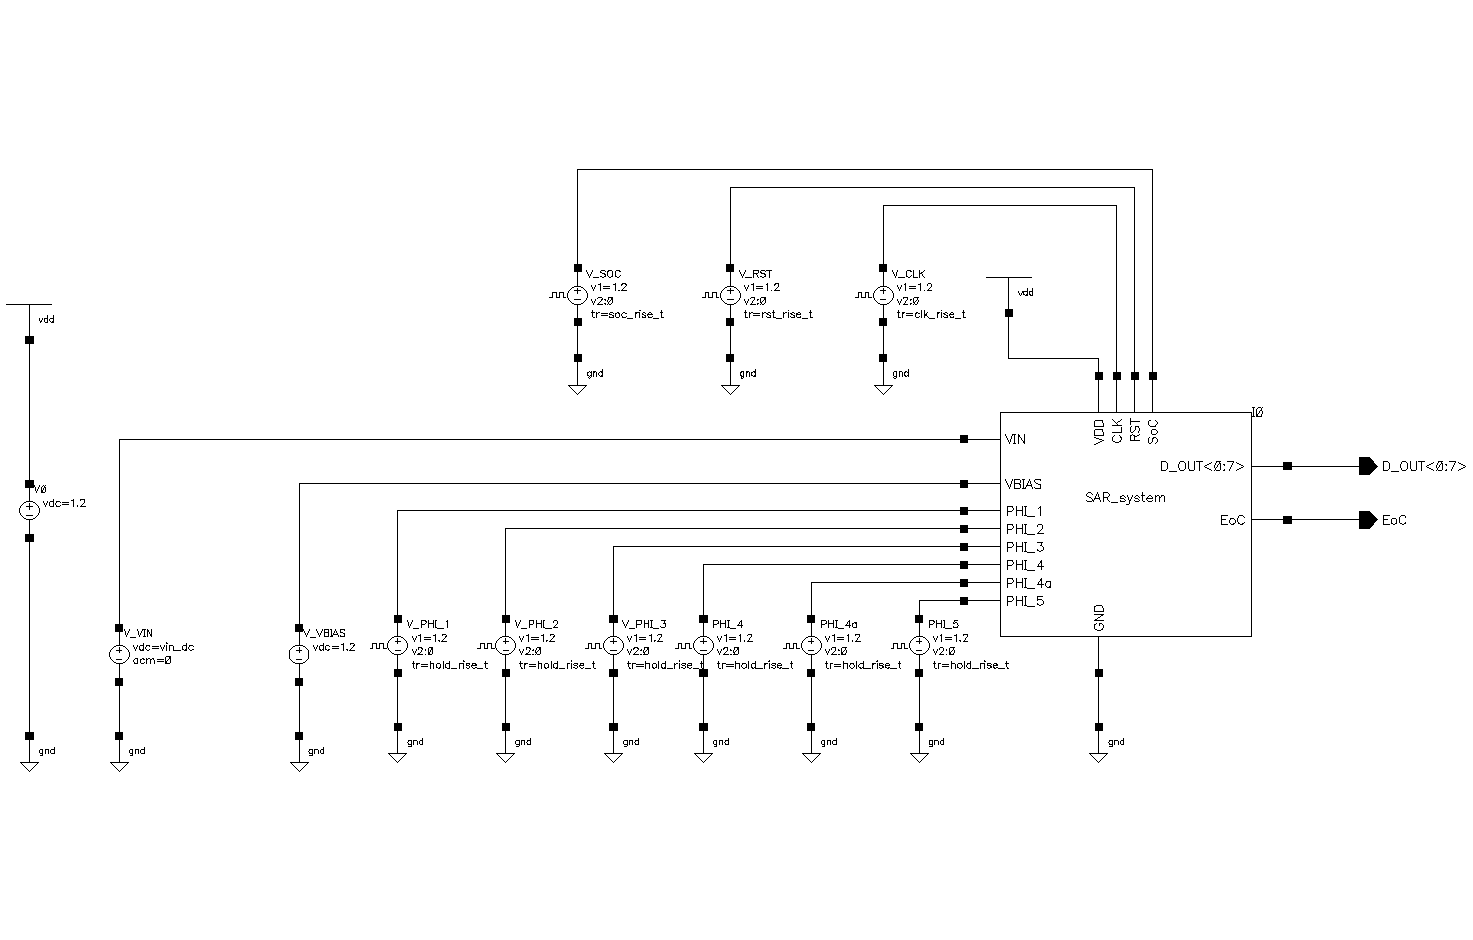
\includegraphics[width=\textwidth]{img/SIM_system.png}
   \caption{Test bench for SAR-ADC circuit}
   \label{sim:system}
\end{figure}
This is a complete system test bench.Here all the different components come together to form the full SAR-ADC architecture.\\ 
\\
Testing on a system level is necessary to ensure that the circuit performs according to the interface the circuit provides to the outside world.\\
\\
This test scenario is quite hard to set up since many signals have to be timed to each other. The verification of the circuit is also challenging since many signals has to be considered.
In order to manage this test we need to generate a test procedure with the specified stimuli and check the results to a expected pattern.
See Figure \ref{sim:system}.

\section*{Schematic: SIM\_sample\_hold}
\begin{figure}[!ht]
 \centering
   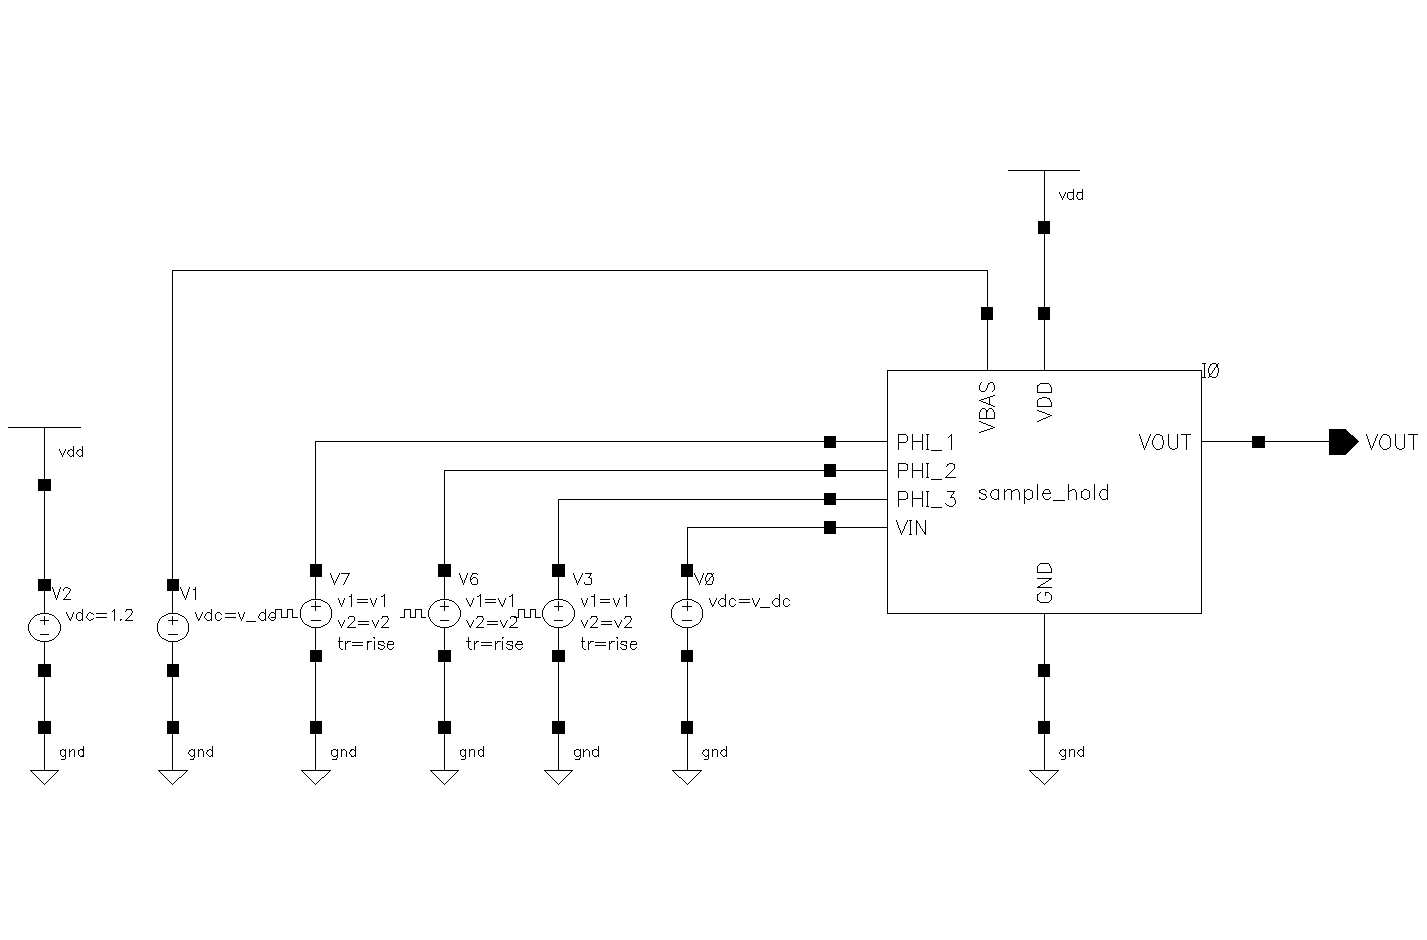
\includegraphics[width=\textwidth]{img/SIM_sample_hold.png}
   \caption{Test bench for sample and hold circuit}
   \label{sim:sh}
\end{figure}
To test the sample and hold we need to generate 3 clocks (see timing diagram in figure \ref{timing}). 
The output is ideally expected to match the input value and hold it in the phi\_3 phase.
See Figure \ref{sim:sh}.

\section*{Schematic: SIM\_comparator}
\begin{figure}[!ht]
 \centering
   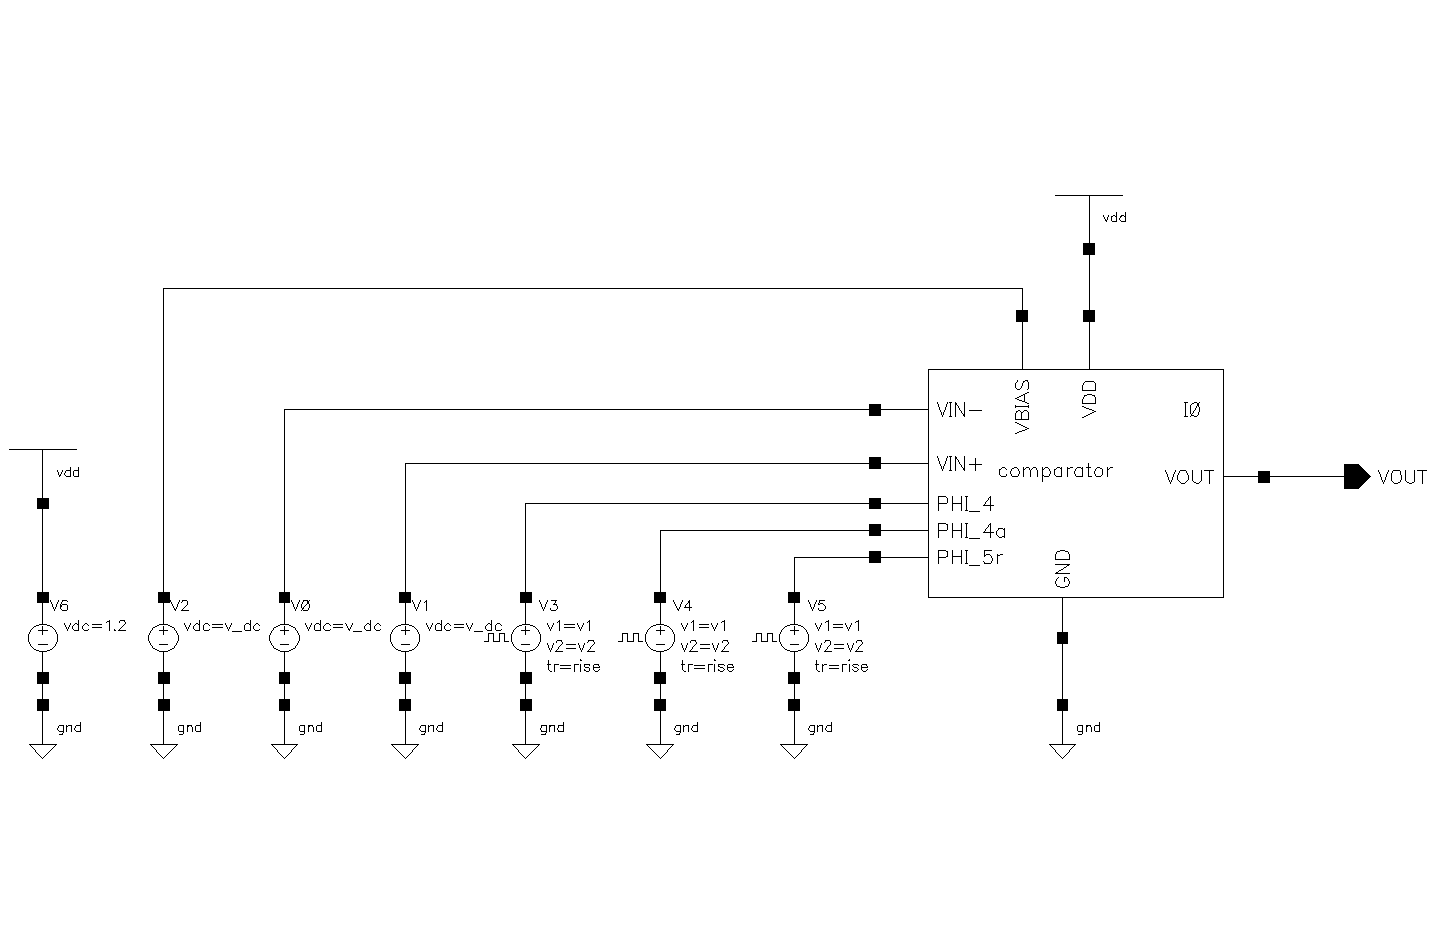
\includegraphics[width=\textwidth]{img/SIM_comparator.png}
   \caption{Test bench for comparator circuit}
   \label{sim:comparator}
\end{figure}
In the test bench for the comparator we need 3 clocks for the timing. 
When sweeping the input (let's say VIN-) we expect that at some point (dependent on VIN+,) that the comparator will change state. 
See Figure \ref{sim:comparator}.

\section*{Schematic: SIM\_SAR\_logic}
\begin{figure}[!ht]
 \centering
   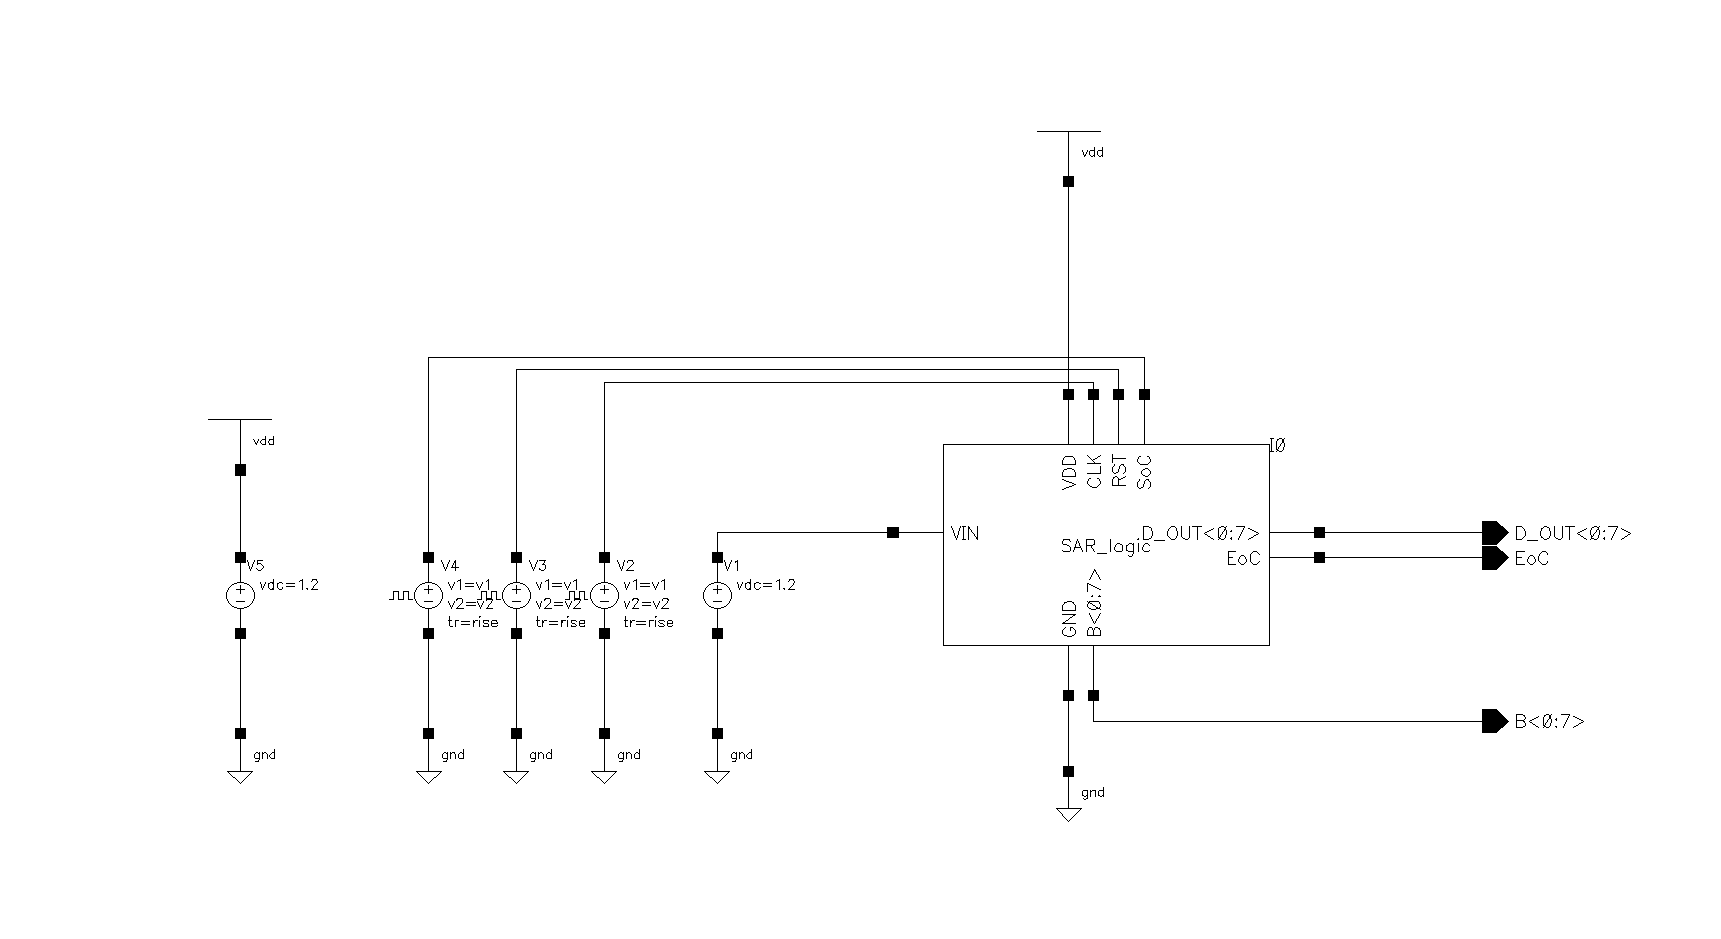
\includegraphics[width=\textwidth]{img/SIM_SAR_logic.png}
   \caption{Test bench for SAR-logic circuit}
   \label{sim:logic}
\end{figure}
Some of the circuit in the SAR-logic is given but some extra circuitry is needed. In this test bench we want to test
that the acquisition state is started when the SoC signal is pulsed. And that we receive a EoC after N-bits clock pulses.
We also need to test the reset functionality. 
The main function of generating the digital output is easy to test since the input signal decides the value of the current bit.
See Figure \ref{sim:logic}.

\section*{Schematic: SIM\_dac}
\begin{figure}[!ht]
 \centering
   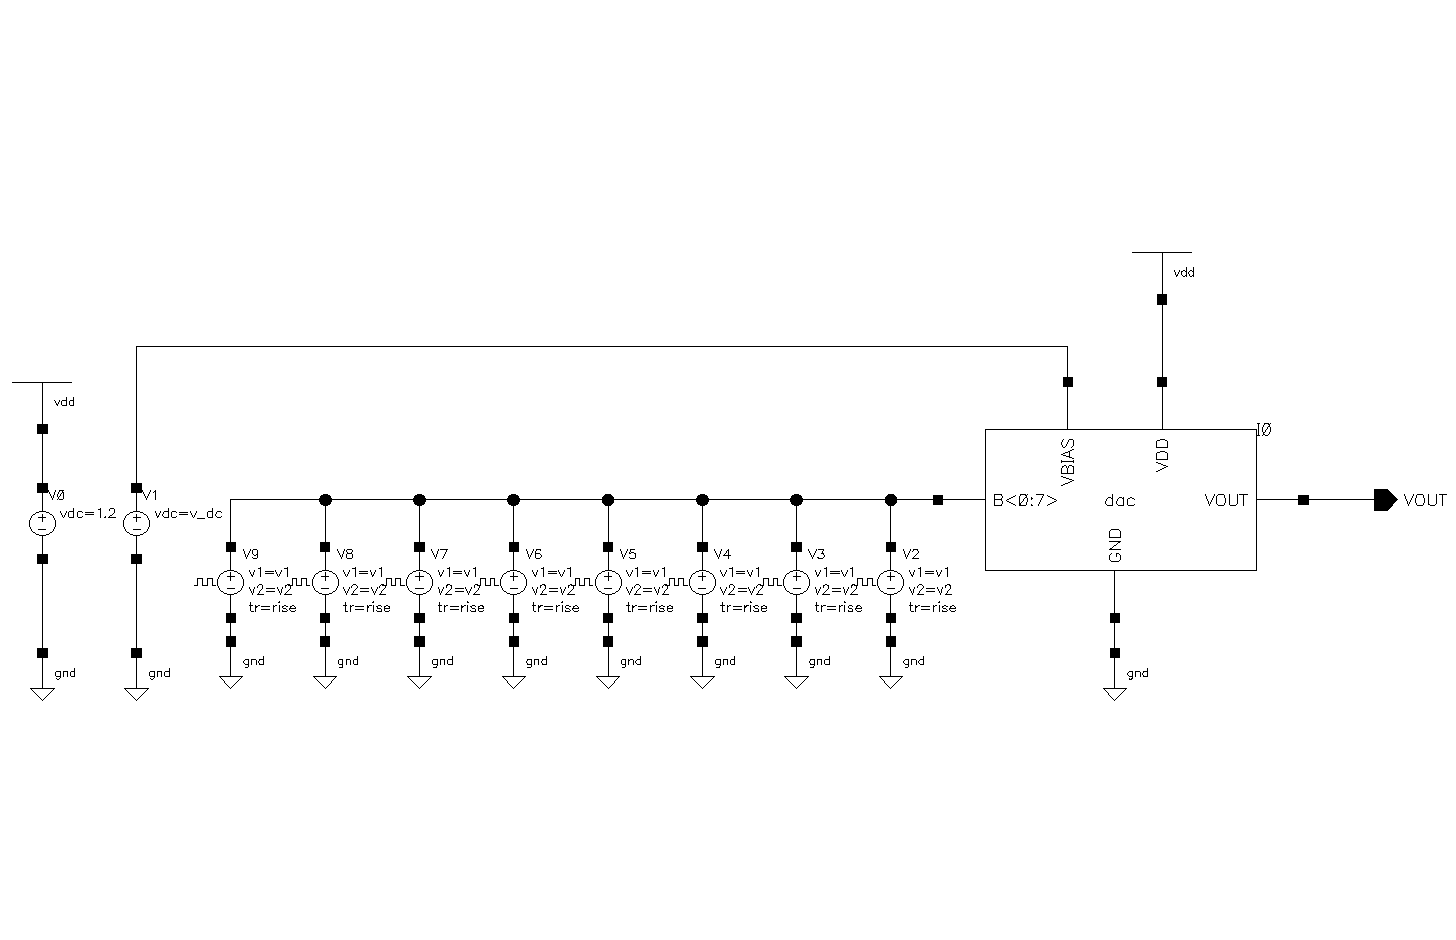
\includegraphics[width=\textwidth]{img/SIM_dac.png}
   \caption{Test bench for DAC circuit}
   \label{sim:dac}
\end{figure}
The test-bench for the DAC consists of N-bits pulse generators so that we can apply a binary pattern. 
VOUT should be proportional to the binary value.
See figure \ref{sim:dac}.

\section*{Schematic: SIM\_op\_amp}
\begin{figure}[!ht]
 \centering
   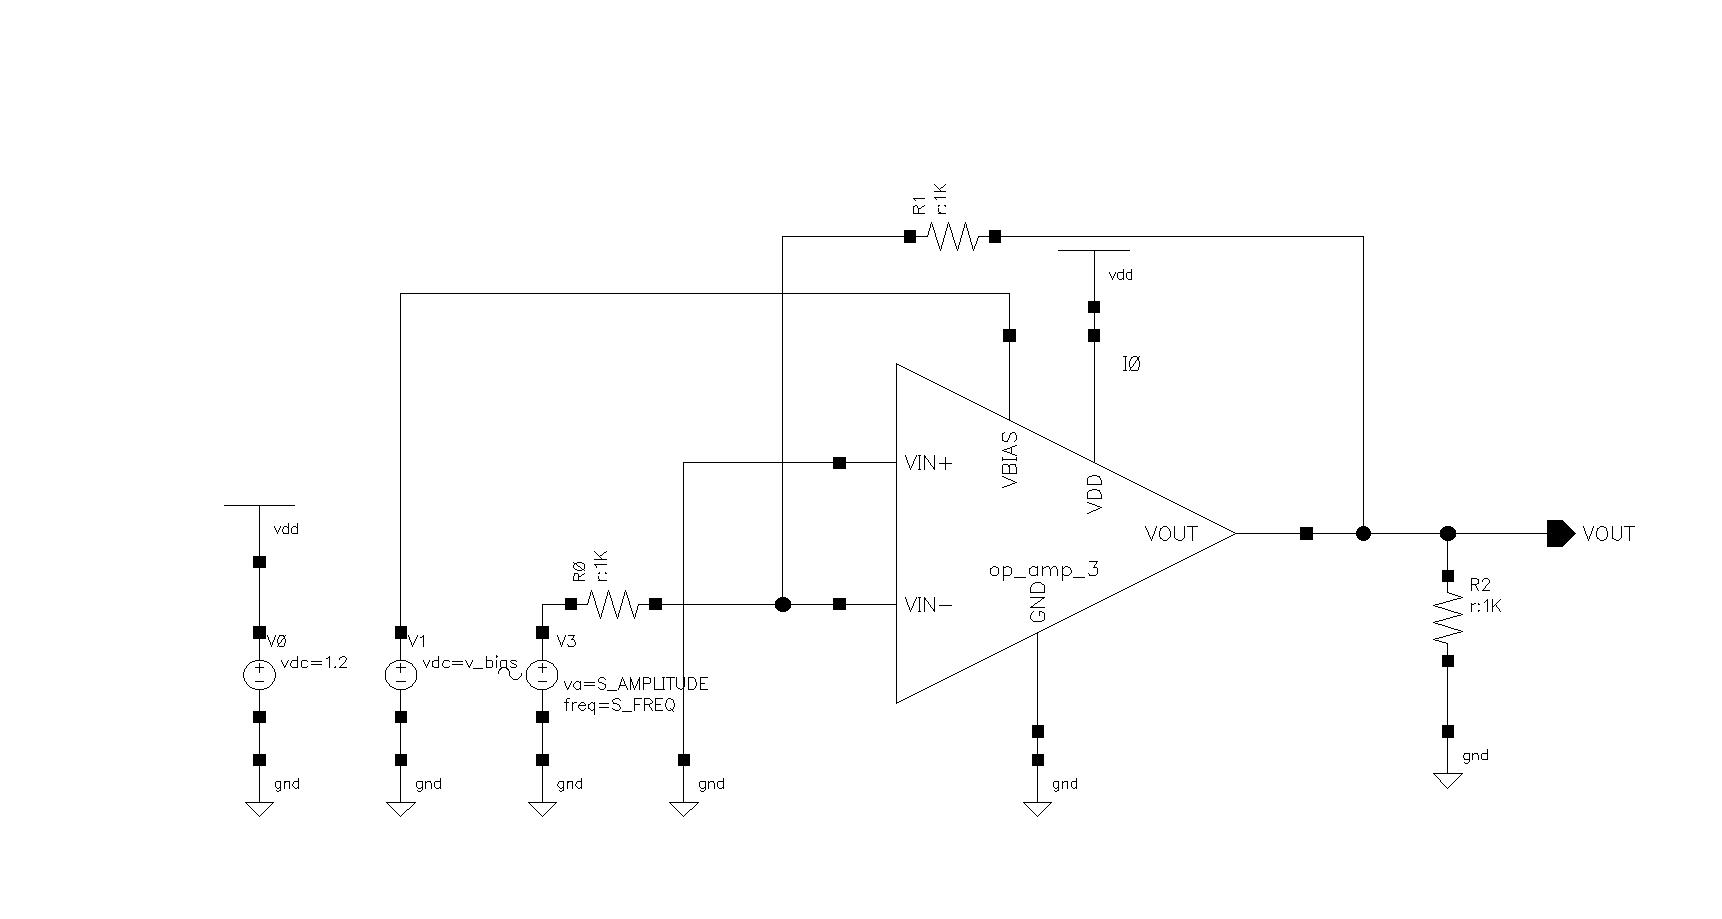
\includegraphics[width=\textwidth]{img/SIM_op_amp_3.png}
   \caption{Test bench for op-amp circuit}
   \label{sim:opamp}
\end{figure}
In our test bench for the op-amp we have an open circuit amplifier that expect is going to saturate to either (almost) GND or VDD, if our gain is high enough.
This simulation is a test to check for response and not performance.
This simple test gives little information about the performance of the op-amp. 
To get a better test of the performance of the circuit we need more tests where we test other configurations of the op-amp. 
See Figure \ref{sim:opamp} and \ref{sim:opamp_ac_responce_and_bode_plot}.

\begin{figure}[!ht]
 \centering
   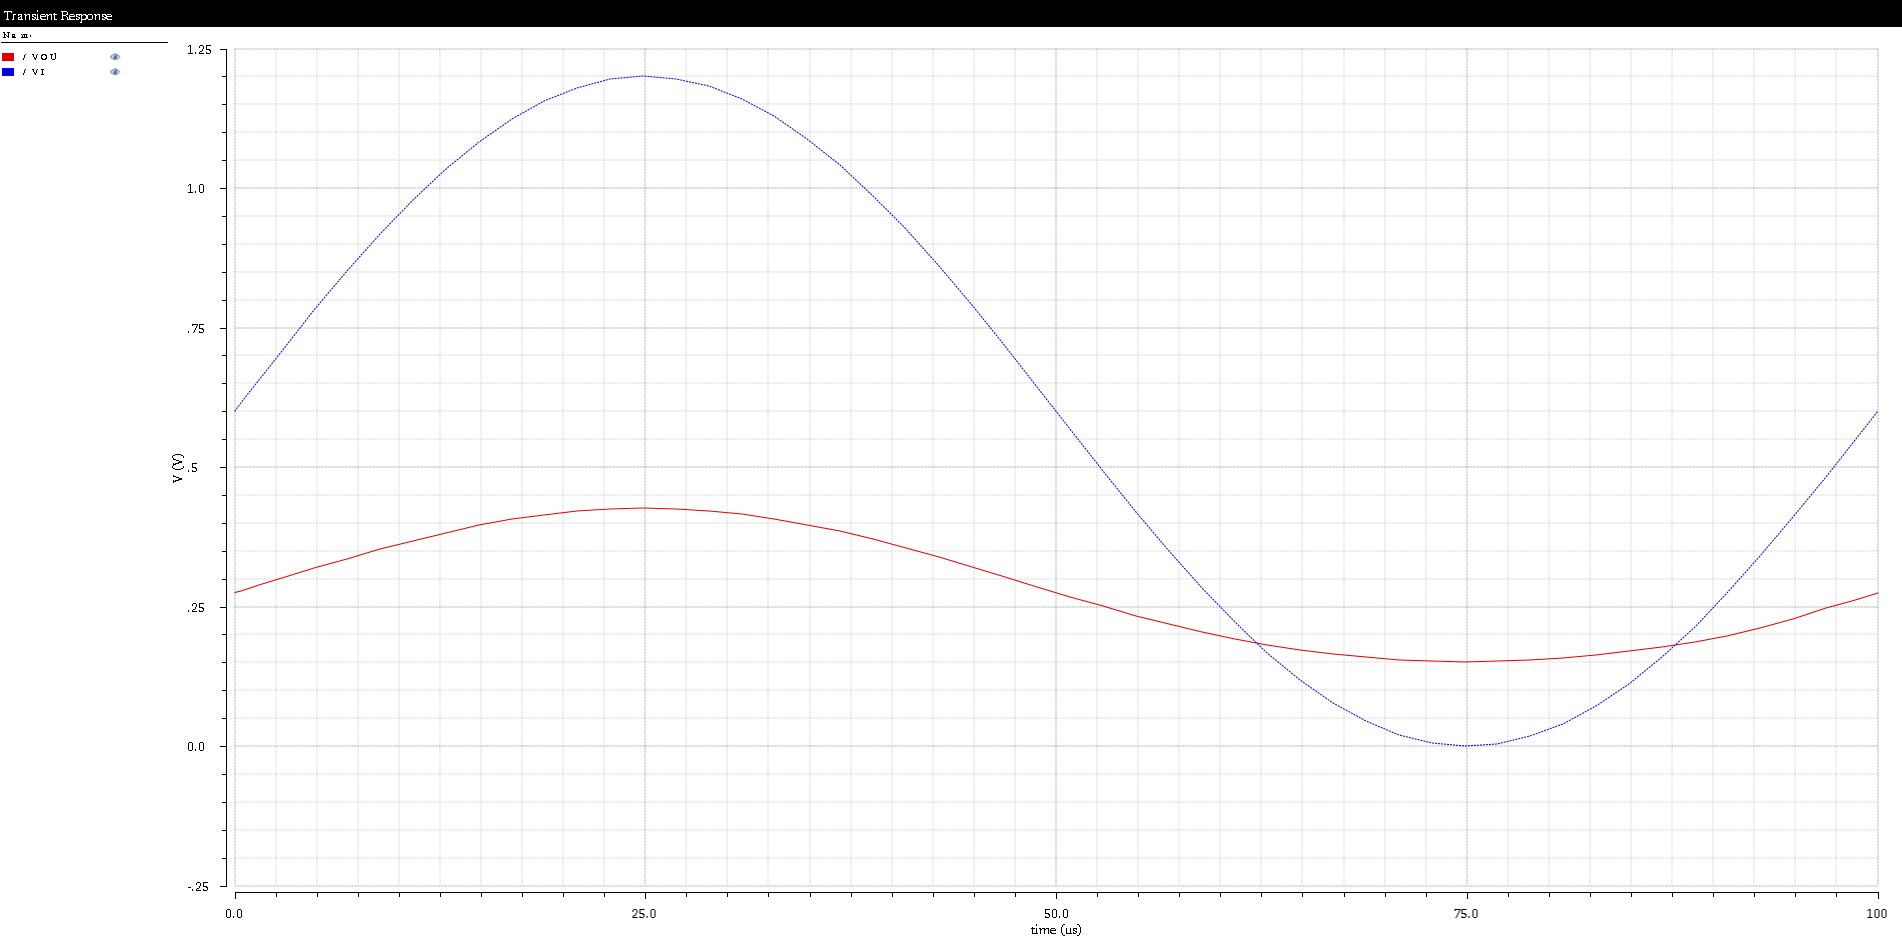
\includegraphics[width=0.75\textwidth]{img/ac_responce_and_bode_plot.png}
   \caption{AC response from op-amp circuit used as a non-inverting amplifier}
   \label{sim:opamp_ac_responce_and_bode_plot}
\end{figure}

\newpage
\printbibliography{}
\end{document}
